%\documentclass[tikz,convert={outfile=\jobname.svg}]{standalone}
\documentclass[tikz,convert={outfile=\jobname.png}]{standalone}
%\documentclass{standalone}

\usepackage{tikz}
\begin{document}

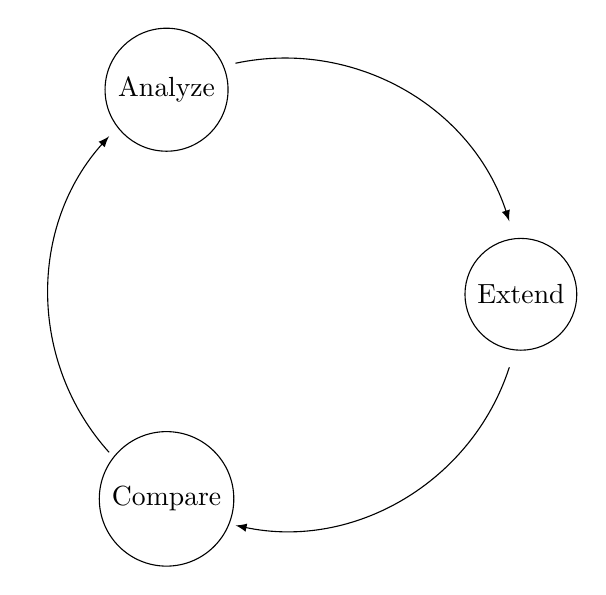
\begin{tikzpicture}
\def \n {3}
\def \radius {3cm}
\def \margin {18} % margin in angles, depends on the radius


\node[draw, circle] at ({360/3 * 2}:\radius) {Compare};
\draw[->, >=latex] ({360/\n * 3 - \margin}:\radius)
  arc ({360/\n * 3 - \margin}:{360/\n * 2 + \margin}:\radius);

\node[draw, circle] at ({360/3 * 1}:\radius) {Analyze};
\draw[->, >=latex] ({360/\n * 2 - \margin}:\radius)
  arc ({360/\n * 2 - \margin}:{360/\n * 1 + \margin}:\radius);

\node[draw, circle] at ({360/\n * 0}:\radius) {Extend};
\draw[->, >=latex] ({360/\n * 1 - \margin}:\radius)
  arc ({360/\n * 1 - \margin}:{360/\n * 0 + \margin}:\radius);




%\foreach \s in {1,...,\n}
%{
%  \node[draw, circle] at ({360/\n * (\s - 1)}:\radius) {$\s$};
%  \draw[->, >=latex] ({360/\n * (\s - 1)+\margin}:\radius) 
%    arc ({360/\n * (\s - 1)+\margin}:{360/\n * (\s)-\margin}:\radius);
%}
\end{tikzpicture}

\end{document}
